\section{Belt Drive}\label{sec:belt_drive}
\subsection{Description}
Synchronous belt drive systems are said to be efficient, reliable, virtually maintenance free and are supposed to outlast any comparable chain drive system. The system used on this vehicle consists of a Gates PowerGrip GT3 belt which is rated for high torque transmission at variable speeds while the sprockets and accompanying bushings were supplied by Martin Sprocket for cost saving reasons.

\begin{table}[htbp]
	\centering
	\caption{Belt Drive Component Summary}
	\begin{tabular}{| lll |} \hline
		Component & Manufacturer & Description \\ \hline
		\multirow{4}{*}{Belt} & \multirow{4}{*}{Gates} & Gates PowerGrip GT3 \\
		& & 225 teeth \\
		& & 8 mm pitch \\
		& & 30 mm pitch \\ \hline
		\multirow{2}{*}{Large Sprocket} & \multirow{2}{*}{Martin Sprocket} & 72 teeth\\
		& & Steel \\ \hline
		\multirow{2}{*}{Large Bushing} & \multirow{2}{*}{Martin Sprocket} & 2517 Style Taper-Lock Bushing\\
		& & Steel \\ \hline
		\multirow{2}{*}{Small Sprocket} & \multirow{2}{*}{Martin Sprocket} & 44 teeth\\
		& & Steel \\ \hline
		\multirow{2}{*}{Small Bushing} & \multirow{2}{*}{Martin Sprocket} & 2012 Style Taper-Lock Bushing\\
		& & Steel \\ \hline
	\end{tabular}
	\label{tab:drive_comp}
\end{table}

\begin{figure}[h]\centering
	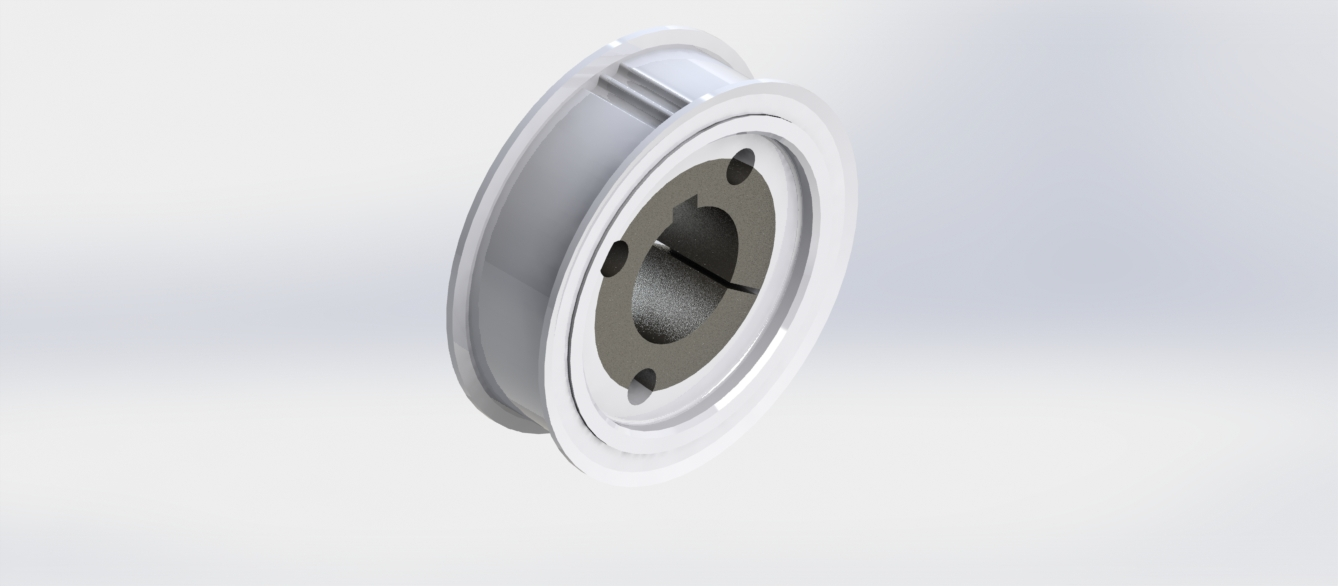
\includegraphics[width=.7\linewidth]{dom/small_sprocket_with_bushing_rndr.jpg}
	\caption{Small Sprocket}
	\label{fig:small_sprocket}
\end{figure}

\subsection{Design Constraints and Functional Requirements}
The overall width of belts and sprockets proved to be a considerable constraint in itself. While there was a specific width required to ensure power transmission without failure, this same width also hindered the design of the drive box as it would result in a thicker and bulkier design. The engineers at Gates were consulted regarding optimization of belt width and sprocket diameters. After a couple weeks of back and forth by email, it was decided that a 30mm wide belt would be best suited.

Next constraint proved to be the diameters of the sprockets as there was an overall size constraint of the drive box. It should also be noted that larger diameters lead to a substantial increase in weight and cost. Therefore finding the happy-medium between required diameter for belt life, overall size, weight and cost was a challenge. There was also the ratio between diameters of the driving sprocket and idlers that needed to remain constant. This ratio, determined by required output speeds and torque transmission, was found to be 1.6.

The position of the idler was also a challenge due to dimensional constraints imposed by the location of the small and large sprockets and ensuring sufficient wrap angle on the driving sprocket. A constraint that wasn’t discovered until part sourcing began was the availability of the sprocket diameters and material selection for these. This proved to be the biggest constraint to overcome since all of those mentioned above also came into play with this constraint.

The goal of the belt drive is to have an efficient and reliable power transmission method that requires minimal maintenance and is easy to assemble and disassemble. Lower operating costs, a dry running drive box and reducing the need for a well sealed drive box are criteria that benefited the design.

\subsection{Analysis and Design}
For the design of the belt system, calculations were done following the design procedure in the Gates PowerGrip GT3 Design Manual and results were verified using the Gates Design IQ software. Using a maximum torque output from the motors of 156 N-m (at 1.2 HP) with an output speed of 60 rpm, a required belt width of 30mm was calculated both by hand and using the software with sprockets having an acceptable size of 72 teeth for the large sprocket and 44 for the small sprocket. A triple check was conducted by the engineers at Gates. They were provided all the details mentioned above and conducted their separate analysis using different software to confirm the results. 

It is important to mention that the belt system will be alternating from clockwise rotation to counterclockwise rotation. This was discussed with the engineers at Gates and they confirmed that since a robust slotted idler is being used, the change between slack and tight side shouldn’t be an issue for this system.